% ============================================================================ ARCHITECTURES + MODELS
\section{Integration Architectures and Physical Models}\label{sec:models}

\subsection{Three integrations of one regulator}\label{sec:archs}
The synthesized regulator of Section~\ref{sec:dse} is placed in three integrations
(Fig.~\ref{fig:sections}). All three hold the same \MthNcells{} cells on a
$\MthGrid\times\MthGrid$ grid under the 22.36-mm die, each cell \MthCellSide~mm square at a
\MthCellPitch-mm pitch. They share one converter stack, one tier order and one
\MthBoardMm-mm board, so they differ in placement only (layer stacks: Table~S4).

In the \emph{embedded} integration (Z1), the \MthStackMm-mm converter sits between a
300-\textmu m silicon power substrate and the die. Its 48-V input crosses the board, the 48-V
balls of the BGA, a 48-V RDL on the substrate and the TSVs. Its 1-V output reaches the die through a 10-\textmu m output RDL
and the die pads.

In the \emph{package-backside} integration (Z2), the converter hangs below the substrate inside
a \MthCutout-mm opening in the board, 1~mm from the sidewall. A 30-\textmu m attach of
15-\textmu m Cu pillars at 30-\textmu m pitch joins it to the substrate; thermocompression
bonding at that pitch has been demonstrated on organic substrates~\cite{Au2016CuPillar30um}.
Only the 1-V current crosses the attach and the TSVs. The BGA is a ring of \MthSitesRing{}
sites around the opening, and its power balls carry the 48-V feed. The feed current runs from
the board through these balls and a 48-V RDL on the land side of the substrate to the input pads
of the cells. The lowest face of the converter lies \MthClearZtwo~\textmu m above the underside of
the board.

In the \emph{board-backside} integration (Z3), the converter is attached to the underside of an
uncut board beneath the package, as in current vertical power modules~\cite{Vicor_VPD_AI}. Its
1-V output crosses a board-level solder attach, a field of plated through-holes in the board,
the full BGA and the TSVs. A pair of 48-V copper planes in the board feeds it, and a second cold
plate cools it from below.

\begin{figure*}[!t]
\centering
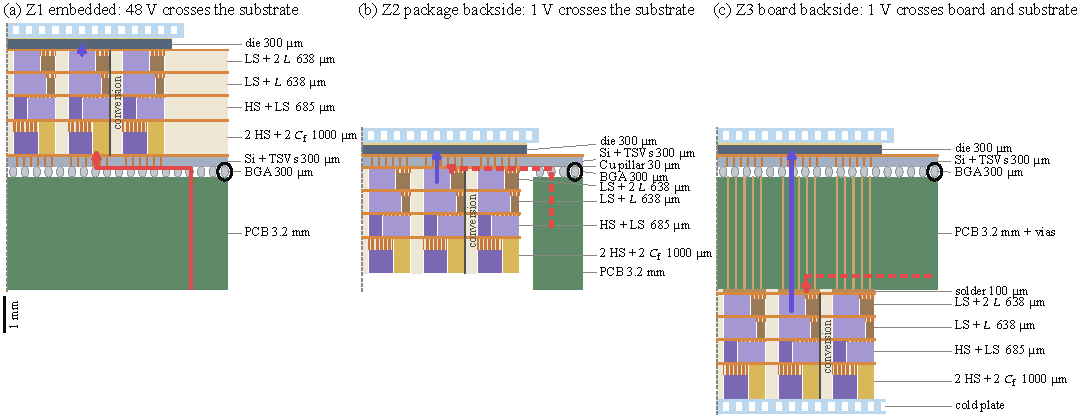
\includegraphics[width=\textwidth]{fig3_sections.pdf}
\caption{The three integrations as meshed: half sections, to scale in $z$ (10-\textmu m RDLs
drawn as lines). Every converter tier holds the parts of its design-record tier; copper posts
(hatched) fill the height above parts shorter than the tier. (a) Z1: converter between
substrate and die, full BGA. (b) Z2: converter in the board opening below the substrate; its
48-V feed runs through the BGA ring and the substrate (dashed). (c) Z3: converter on the board
underside with its own cold plate; the full BGA carries the 1-V output. Red: 48-V path; violet:
1-V path; ringed ball: the outermost row, which holds the critical (corner) joint in every
compared case.}
\label{fig:sections}
\end{figure*}

\subsection{Converter stack, tier order and vertical interconnect}\label{sec:realizability}
The parts of a cell are packed into at most four tiers, and a tier may mix part classes
(Section~\ref{sec:dse}). Each part keeps its body footprint and a \MthKeepout-\textmu m keep-out
in a two-dimensional placement. Listed from the 48-V input end, the first tier holds two
HS dies and both flying capacitors (\MthTierOne~\textmu m). The second holds an HS and an LS die
(\MthTierTwo~\textmu m), the third an LS die and an inductor
(\MthTierThree~\textmu m), and the fourth an LS die and two inductors (\MthTierFour~\textmu m).
With its 10-\textmu m interlayer RDLs, the converter is \MthStackUm~\textmu m tall.

A tier is as tall as its tallest part: the rated 0603 capacitor (\MthHtCf~\textmu m maximum
height), the EPC2014C (\MthHtHs~\textmu m with its terminals) or the EPC2055
(\MthHtLs~\textmu m). Copper posts on the terminals bridge every shorter part to the RDLs above
and below it. They are sized to each die's datasheet land pattern, to the electrode bands of the
capacitor and to the inductor current at 100~A\,mm$^{-2}$. We assume dies with terminals on both
faces, so a die connects through the capture planes on both sides of its tier; single-face
terminals are treated as a sensitivity below.

Whether two parts in different tiers can be connected depends on the conductor planes between
them. An interlayer RDL is patterned copper and serves as a capture plane, so a via must cross
only the dielectric depth of the tiers in between. Each vertical net is checked against the via
count of~\eqref{eq:via}, the pitch, the landing area of the part and the aspect ratio of every
via level. The declared rules are those of chip-embedding
substrates~\cite{Ostmann2008ChipEmbedding}. Laser-drilled \MthViaD-\textmu m microvias cross a
build-up dielectric, every RDL carries a capture pad 1.5 times the via diameter, and each via
level has an aspect ratio of at most 1. This limit is the stacked-microvia practice of
high-density boards~\cite{IPC2226A2017,Ning2019MicroviaFatigue}.

The tier order is chosen in three steps. First, only orders that meet the via rule are kept; if
none does, the orders with the best worst-case aspect ratio are kept. Second, the order of least
intra-cell routing loss is taken. This loss uses the conductor model of the ledger at
25\,$^\circ$C, with the bare input factor on the 48-V nets (Sections~\ref{sec:scenarios}
and~\ref{sec:ledger}). Each order carries the assignment of parts to tiers that routes with the
least loss. Third, orders within \MthRouteTie~W of the least loss are separated by their heat
path, a one-dimensional estimate of the temperature rise from each tier's loss to the die-side
face.

None of the \MthNorders{} orders of the four tiers meets the via rule (Fig.~\ref{fig:realize}).
Every order must cross the \MthTierOne-\textmu m capacitor tier, so its worst via level has an
aspect ratio of \MthWorstAR. That crossing therefore needs copper posts, not build-up vias. The
least routing loss is \MthRouteLeast~W, and \MthNtie{} orders lie within \MthRouteTie~W of it.
Among them the heat path selects the order listed above. It routes \MthRouteChosen~W inside
the cells and has a \MthHeatChosen-K heat path, against \MthHeatLeast~K for the least-loss
order. The same order with its worst part assignment would route \MthRouteWorst~W. Regrouping
the parts into every packable set of at most four tiers (\MthNgroupings{} groupings, \MthNregroup{}
orders) does not remove the posts either: the best worst-case aspect ratio is \MthRegroupAR.

Two sensitivities test this verdict. With a 100-\textmu m capacitor tier the stack shrinks to
\MthThinStackMm~mm, but every order still crosses a device tier, at an aspect ratio of at least
\MthThinAR. With single-face terminals the rule selects the same order, and its worst aspect
ratio stays \MthSingleAR. The verdict is geometric feasibility under declared rules, not a
demonstrated process. Placement within a tier, encapsulation and warpage during lamination are
not evaluated (Section~\ref{sec:discussion}).

The four-tier limit also constrains the converter. The five-tier optimum at the same count
($N4K4$, \MthFswFive~kHz) has a lower electrical loss but a \MthStackFiveMm-mm stack. Hung in the
opening of Z2, it would protrude \MthProtrude~\textmu m below the board
(Section~\ref{sec:explore}).

\begin{figure}[!t]
\centering
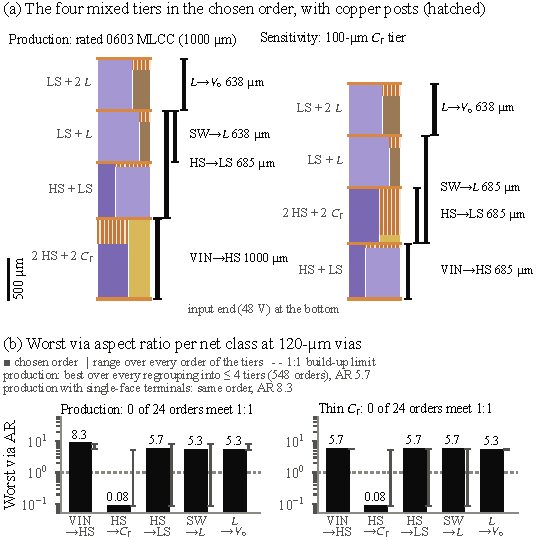
\includegraphics[width=\columnwidth]{fig4_realizability.pdf}
\caption{Tier order as a realizability constraint. (a) The four mixed tiers in the chosen
order, to scale, with the rated 0603 capacitor (production, \MthTierOne-\textmu m tier) and with
a 100-\textmu m capacitor tier (sensitivity); copper posts (hatched) fill the height above
shorter parts, and a bar marks each net class that must cross a whole tier. (b) Worst via
aspect ratio per net class at \MthViaD-\textmu m vias against the 1:1 build-up limit. No order
of either stack meets it, so copper posts make every whole-tier crossing.}
\label{fig:realize}
\end{figure}

\subsection{Input states}\label{sec:scenarios}
The hybrid cell draws input current only in phase $\phi_1$ (Fig.~\ref{fig:converter}b). The RMS
current of the 48-V path therefore depends on how much of that pulse local decoupling absorbs.
We describe it by the RMS factor $k_{\mathrm{rms}}$, the ratio of the RMS to the average 48-V
current. Three input states bound it. \emph{Ideal decoupling} ($k_{\mathrm{rms}} = 1$) is the
limit of unlimited local capacitance. \emph{Bare decoupling} passes the pulse at the buck duty
$D$ unfiltered, $k_{\mathrm{rms}} = 1/\sqrt{D} = \MthKbare$. \emph{Implemented decoupling} is
the production state. Its \MthNphases{} clock phases run in two interleaved groups of six, and a
ring of \MthNring{} 1206 capacitors sits outside the cell grid. Together they give
$k_{\mathrm{rms}} = \MthKeq$ in the package network (Section~\ref{sec:evaluate}). The input
loop inside each cell still carries the bare pulse of the cell, $k_{\mathrm{rms}} = \MthKcell$
from a circuit model of its waveform. Ideal and bare decoupling serve as references.

\subsection{Rail-aware conductor ledger}\label{sec:ledger}
Loss is reported inside a declared boundary. The package-internal loss $P_{\mathrm{int}}$ of Z2
and Z3 starts at the 48-V input terminals of the converter. That of Z1 starts at its 48-V BGA
pads, where the 48-V node of the board, common to all three, meets the package. The board's 48-V
distribution upstream of that node is common to all three and excluded. The external feed of a
backside integration, from that node to the converter, has the loop resistance $R$ and costs
\begin{equation}
P(R) = P_{\mathrm{int}} + \left(k_{\mathrm{rms}} I\right)^2 R,\qquad
V_{\mathrm{in}}\, I = P_{\mathrm{load}} + P(R),
\label{eq:feed}
\end{equation}
where $V_{\mathrm{in}} = 48$~V, $P_{\mathrm{load}} = 1$~kW, $I$ is the average input current and
$k_{\mathrm{rms}}$ the RMS factor of the current the feed carries. Equation~\eqref{eq:feed} is
solved for $I$ by fixed-point iteration. The feed loss is dissipated outside the package and is
not deposited in its thermal model. The same factor scales the package 48-V network of Z1: the
pulsed input current is charged wherever it flows. The crossover $R^{\ast}$ at which a backside
integration loses its advantage over Z1 is a specification for the feed. Two physical feeds are
evaluated against it. The ring feed of Z2 is solved with the same network model as Z1, a
\FeedRbgaZtwo-m$\Omega$ loop. The plane pair of Z3 is two \MthFeedPlaneT-\textmu m copper planes
under the cell grid, a \FeedRZthree-m$\Omega$ loop.

Every conductor carries the rail assigned to it and the RMS current that flows in it. Switched
nets inside the cell carry the RMS currents of the converter model, and the 48-V nets carry
$k_{\mathrm{rms}} I$. The 1-V path carries the RMS cell output current, \MthIoutRatio{} times its
\MthIcell-A average. A vertical field of vias of radius $r$, liner $t_\ell$ and height $h$
carrying the current $I$ is provisioned at a design current density $J_{\mathrm{d}}$ and resolved
by its allocated count,
\begin{equation}
\begin{aligned}
n_{\mathrm{req}} &= \left\lceil \frac{I}{J_{\mathrm{d}}\pi(r-t_\ell)^2}\right\rceil \le
n_{\mathrm{alloc}} \le n_{\mathrm{avail}},\\
R &= \frac{\rho(T)\,h}{\pi(r-t_\ell)^2\,n_{\mathrm{alloc}}},
\end{aligned}
\label{eq:via}
\end{equation}
where $r-t_\ell$ is the copper radius inside the liner, $\rho(T)$ the copper resistivity at the
converged temperature of the field and $n_{\mathrm{avail}}$ the count the pitch rule fits in the
footprint. Inside the cell $J_{\mathrm{d}} = 100$~A\,mm$^{-2}$. Contact and intermetallic
resistances at via and joint interfaces are not resolved; the attach and pad terms carry them
as an all-solder bound. A lateral run is a sheet whose required width must fit the available
width. A link between parts in different tiers is a via stack across the actual tier order, a
link within a tier is a lateral run, and the output plane of the cell is a finite-volume sheet.

Under each cell, \MthTsvCell{} TSVs of 30~\textmu m at 60-\textmu m pitch carry 48~V in Z1 and
1~V in Z2 and Z3. The package 48-V network of Z1 and the ring feed of Z2 are each solved as two
voltage-fed resistive sheets, supply and return. Every ball and pad feeds the sheets through its
own resistance, on a finite-volume grid aligned with every pad and ball edge. The ball currents
are therefore an output. The Cu-pillar attach of Z2 (\MthPillarCell{} pillars per rail and cell)
and the solder attach of Z3 (\MthZthreeBumps{} bumps per rail and cell) are resolved on their
lattices as series columns with two-sided constriction. In Z3, \MthPthCell{} plated
through-holes per rail and cell carry the 1-V current through the board.

The 48-V balls of Z1 and of the ring of Z2 are provisioned by one rule. The current of a ball is
the largest DC ball current of the solved network, scaled by $k_{\mathrm{rms}}$. The count is the smallest
legal (mirror-symmetric) count on the 0.8-mm lattice that holds this current to
\MthBgaTarget~A per ball. This target is a design assumption for 0.4-mm SAC305 (Sn3.0Ag0.5Cu)
balls~\cite{Kuan2015Imax}. A conservative \MthBgaTargetSens-A target is a sensitivity (Section~\ref{sec:explore}).
The power balls may occupy at most \MthLimSites~\% of the sites of the package; the rest carry
signal and auxiliary rails. The harmonic port model of Z1, with every ball tied to an ideal board
node, bounds its worst ball at \MthBgaRmsBound~A RMS. This bound exceeds the target and is
discussed as a limitation (Section~\ref{sec:discussion}).

In Z3 the 1-V current of each rail is shared equally by balls that cover most of the BGA, while
the TSV fields that carry it to the die sit only under the cells. The current of every ball
outside a cell footprint therefore travels laterally, in a land-side copper plane of the
substrate and in the 1-V planes of the board. Each sheet costs
\begin{equation}
\begin{aligned}
P &= \kappa\, R_{\mathrm{s}}(T)\, I_{\mathrm{r}}^2,\qquad
\Delta V = \kappa_V R_{\mathrm{s}}(T)\, I_{\mathrm{r}},\\
R_{\mathrm{s}}(T) &= \rho(T)/(\varphi\, t_{\mathrm{Cu}})
\end{aligned}
\label{eq:sheet}
\end{equation}
for a rail current $I_{\mathrm{r}}$, where $\kappa$ and $\kappa_V$ are shape factors, $t_{\mathrm{Cu}}$
the copper thickness and $\varphi$ its occupancy. The shape factors come from a two-dimensional
finite-volume solution of one rail's sheet. Equal ball currents are its sources, and the TSV or
via fields under the cells are its sinks. Halving its \MthLandGrid-mm grid changes them by
\MthLandGridChk~\%. The land side gives $\kappa = \MthLandKappa$ per rail at
$t_{\mathrm{Cu}} = \MthLandT$~\textmu m and $\varphi = \MthLandOcc$~\%. The board planes are
\MthPlaneN{} declared \MthPlaneT-\textmu m planes per rail at $\varphi = \MthPlaneOcc$~\%, with
$\kappa = \MthPlaneKappa$ for both rails together. Each $R_{\mathrm{s}}$ is evaluated at the
converged temperature of its layer, and the redistribution heat is deposited along its
finite-volume loss map.

\subsection{Package thermal model and cooling}\label{sec:thermal}
Steady conduction $\nabla\!\cdot(\mathbf{k}\nabla T) + q''' = 0$ is solved on the explicit
stack with orthotropic conductivity. Layers that contain regular arrays (TSV fields, attaches,
RDL tiers, ball fields and the board via field of Z3) carry homogenized tensors, each checked
against an explicitly meshed unit cell (Section~\ref{sec:verification}). Every ledger term is
deposited in the layer and cell footprints that produce it. The deposited heat equals the
ledger total to round-off, a relative $\MthDepositResid$.

Each converter tier carries a card homogenized on a unit cell of its contents. Every part is a
vertical column spanning the tier: a series stack of its own layers and, above a shorter part,
its copper posts in encapsulant. The columns and the encapsulant act in parallel through the
thickness; in plane, the midpoint of the series--parallel bracket is used. The posts raise the
through-thickness conductivity of the input-end tier from \MthKzTierOneEncap{} to
\MthKzTierOne~W\,m$^{-1}$K$^{-1}$, and across the four tiers it lies between \MthKzLo{} and
\MthKzHi~W\,m$^{-1}$K$^{-1}$. Sizing the posts to the terminal RMS currents (lower bound) or to
the terminal outlines (upper bound) spans \MthKzPostLo--\MthKzPostHi~W\,m$^{-1}$K$^{-1}$; both
bounds are run as variants (Section~\ref{sec:explore}).

The top boundary is a silicon microchannel cold plate (Table~S5) on a 50-\textmu m thermal
interface material (TIM; 3~W\,m$^{-1}$K$^{-1}$, \TimH~kW\,m$^{-2}$K$^{-1}$). Its effective coefficient
follows from the channel geometry and the flow,
\begin{equation}
\begin{aligned}
h_{\mathrm{eff}}^{-1} &= A_{\mathrm{f}}\left(R_{\mathrm{conv}} + R_{\mathrm{base}}\right),\quad
R_{\mathrm{conv}} = \frac{1}{h_{\mathrm{ch}}\Lambda A_{\mathrm{f}}},\\
\Lambda &= \frac{n L_{\mathrm{ch}}(w + 2\eta_{\mathrm{f}}H)}{A_{\mathrm{f}}},\quad
h_{\mathrm{ch}} = \frac{\mathrm{Nu}\,k_{\mathrm{f}}}{D_{\mathrm{h}}},\\
\eta_{\mathrm{f}} &= \frac{\tanh(mH)}{mH},\quad
m = \left(\frac{2h_{\mathrm{ch}}}{k_{\mathrm{s}}t_{\mathrm{f}}}\right)^{1/2},
\end{aligned}
\label{eq:heff}
\end{equation}
for $n = 223$ channels of width $w = 50$~\textmu m, depth $H = 300$~\textmu m and length
$L_{\mathrm{ch}} = 22.36$~mm over the footprint $A_{\mathrm{f}}$. The fins are silicon
($k_{\mathrm{s}}$) of thickness $t_{\mathrm{f}} = 50$~\textmu m, $D_{\mathrm{h}}$ is the
hydraulic diameter, $k_{\mathrm{f}}$ the water conductivity, and $R_{\mathrm{base}}$ the
resistance of a 100-\textmu m silicon base. A channel is heated on three walls (the base and both fins)
under the H1 condition, with an adiabatic cover. Its fully developed laminar Nusselt number is
$\mathrm{Nu} = \CoolNu$ at aspect ratio 1/6~\cite{ShahLondon1978,QuMudawar2002}. Water enters
at 25\,$^\circ$C at 27~g\,s$^{-1}$ per plate. Its properties are taken at the mean bulk
temperature, \MthTbulk\,$^\circ$C at 1~kW~\cite{NISTWebBook}. The coolant warming
$T_{\mathrm{f}}(x) = T_{\mathrm{in}} + Q(0\!\to\!x)/(\dot m c_p)$ is resolved along every pass
and iterated with the solid solution. The coefficient therefore excludes the caloric resistance
$1/(2\dot m c_p)$ of a uniform sink, which would count half of the coolant rise twice
(Section~\ref{sec:explore}).

A single 22.36-mm pass would need \CoolDpSinglePass~kPa. The plate is therefore a manifold of
\CoolZones{} streamwise zones with alternating inlet and outlet headers, and each pass is
\CoolPassMm~mm long. The flow is laminar ($Re = \CoolRe$) and is taken as uniform over the
channels and zones. With entrance, plenum, turn and header losses of
handbook order~\cite{Idelchik1996}, the pressure drop is \CoolDp~kPa, \CoolDpRatio{} times
below the single pass. The hydraulic power is \CoolPhyd~W per plate, or
\CoolPshaftLo--\CoolPshaftHi~W at the shaft for pump efficiencies of 0.75 to 0.35. The thermal
entry length (\CoolLth~mm) is \MthLthRatio{} of a pass. The fully developed Nusselt number is
thus a lower bound, and the pass-mean coefficient could be up to \MthNuDevRatio{} times higher.

Cooling~A is this top plate alone. Cooling~B adds an identical plate beneath the cell grid,
behind the same TIM. Its flow is sized so that its coolant rises as much as that of the top
plate: \MthBotFlowZtwo~g\,s$^{-1}$ for the \MthBotQZtwo~W that reach it in Z2. Pumping counts
every plate at its own flow. The die dissipates its 1~kW uniformly; a hot-spot map is a
sensitivity (Section~\ref{sec:explore}). The board is a $30\times30$-mm coupon with natural
convection (10~W\,m$^{-2}$K$^{-1}$) beneath it.

The temperature-dependent terms are iterated with the thermal solution to a fixed point: the
on-resistance of each device, the inductor winding and the resistivity of every conductor. Each
term is evaluated at the mean temperature of the region it is deposited in. Each device sits at
the in-cell temperature of its own tier and uses its own datasheet coefficient. The iteration
stops when every coupled temperature changes by less than 0.25~K and the loss by less than
0.1\,\%. It converges in \MthEtItersLo--\MthEtItersHi{} thermal solves and contracts
geometrically. Each loss change is \MthEtContractLo--\MthEtContractHi{} times the previous one;
the largest factor belongs to \MthEtContractCase. The on-resistance coefficients are fitted to
the datasheet curves over 25--125\,$^\circ$C; above that range they are extrapolated, which the
feasibility stage reports.

\subsection{Thermoelastic package and interconnect search}\label{sec:mechanics}
The converged temperature field loads an FE model of the mounted assembly,
$\boldsymbol{\sigma} = \mathbf{C}:(\boldsymbol{\varepsilon}-\boldsymbol{\alpha}(T-T_{\mathrm{ref}}))$
with $T_{\mathrm{ref}} = 25\,^\circ$C. It uses incompatible-mode hexahedra and cubic silicon;
the board and the ball field are meshed as real layers, and only rigid-body motion is
restrained. With this reference the solution is the change from power-off to the operating
point, the excursion that the local cycle imposes. The moduli and coefficients of thermal
expansion (CTE) are those of Table~S3. The encapsulant between the cells and the thickness and
boundary of the board are declared; their alternatives are rerun on the production mesh
(Section~\ref{sec:explore}).

Every interconnect layer is searched rather than assumed: the BGA, the die microbumps, and the
Cu-pillar attach of Z2 or the solder attach of Z3. At every site of a layer of height $h$, the
shear driver is $\gamma = \Delta u/h$, with the relative in-plane displacement across the layer
\begin{equation}
\Delta u = \left\| \mathbf{u}_{\mathrm{t}} - \mathbf{u}_{\mathrm{b}} \right\|_{xy}
\label{eq:du}
\end{equation}
taken from the nodal displacements on its top and bottom planes, interpolated at the site. The
BGA sites are the \MthSitesFull{} legal sites of the 0.8-mm lattice (\MthSitesRing{} in the
ring of Z2); the thinner layers are evaluated at every mesh node. The BGA joint of largest
$\Delta u$, with the displacement $\du$ at its local temperature $T_{\mathrm{sj}}$, drives the
local submodel. The largest displacement need not give the largest inelastic response, so the
submodel is also solved at competing sites (Section~\ref{sec:verification}).

When the optional interface feedback is enabled, the solved warpage sets the local thickness of
the top TIM. The plate is taken as flat and rigid, resting on the highest point of the warped
die at the nominal 50-\textmu m bond line. The TIM thickens by $g(x,y) = \max u_z - u_z(x,y)$,
so the local coefficient becomes $(h_{\mathrm{eff}}^{-1} + g/k_{\mathrm{TIM}})^{-1}$. The fixed
point and the thermoelastic solution are then iterated until the warpage changes by less than
1\,\%. A conforming TIM ($g = 0$, the production chain) and a rigid plate on the free warpage
bound this feedback.

\subsection{Local solder response}\label{sec:local}
The submodel resolves the critical joint, a 400-\textmu m SAC305 ball 300~\textmu m tall at
0.8-mm pitch~\cite{Krishnakumar2026DVPD}. It is meshed as the equal-area 354.5-\textmu m square
prism between two 20-\textmu m copper pads, on four nested hexahedral meshes (L0--L3). The
lower pad face is fixed. The upper face is displaced in plane by $\du$ (its other components
restrained) for a 300-s dwell at $T_{\mathrm{sj}}$ and returned for a 300-s dwell at
25\,$^\circ$C. Every load change is ramped linearly over 3~s and then held. This prescribed cycle stands in
for power cycling between off and the converged operating point; the thermal transient between
them is not modeled.

The solder is elastic--viscoplastic with $E = 45 - 0.12(T-25)$~GPa. Its room-temperature value is
the midpoint of the band of~\cite{Paska2024SAC305}; the slope, $\nu = 0.36$ and the CTE of
21.5~ppm\,K$^{-1}$ are assumed. The production law adds a temperature-dependent yield stress
with isotropic hardening that saturates at 2\,\% inelastic strain~\cite{Yuan2023SAC305}. Creep of
the overstress follows a Norton law,
$\dot\varepsilon_{\mathrm{in}} = A(T)\langle\sigma_{\mathrm{vm}}-\sigma_y\rangle^{n(T)}$, fitted
to tensile creep data~\cite{Xiao2005SAC} (parameters and sources: Tables~S9 and~S10). Those
data cover 45--150\,$^\circ$C and
\MthCalLo--\MthCalHi~MPa, for a Sn3.9Ag0.6Cu alloy rather than SAC305. Between the 5th and
95th percentiles of dwell time, the joints carry \MthVisHotLo--\MthVisHotHi~MPa hot and
\MthVisColdLo--\MthVisColdHi~MPa cold.
The law is therefore extrapolated in stress, and in temperature below 45\,$^\circ$C during the
cold dwell.

Because the production law is extrapolated, the response is carried as a band over two
laws. The second is the Garofalo law of~\cite{Schubert2003ECTC}, entered as a zero-yield Norton
surrogate refitted at each temperature over the stress window the joints visit. The window and
the responses are iterated to self-consistency; after \MthRefitIters{} fits the window settles
at \MthRefitHotLo--\MthRefitHotHi~MPa hot and \MthRefitColdLo--\MthRefitColdHi~MPa cold. Every
joint-response comparison is judged under both laws (Section~\ref{sec:verification}).

The response is the per-cycle increment of accumulated equivalent inelastic strain on the
stabilized (48th) cycle, volume-averaged over the solder core,
\begin{equation}
\deps = \frac{1}{V_{\mathrm{c}}}\int_{V_{\mathrm{c}}}\!
\left[\varepsilon^{\mathrm{eq}}_{\mathrm{in}}(t_k)-\varepsilon^{\mathrm{eq}}_{\mathrm{in}}(t_{k-1})
\right]\mathrm{d}V,
\label{eq:deps}
\end{equation}
where $t_{k-1}$ and $t_k$ bound the last cycle. The core $V_{\mathrm{c}}$ excludes a band of
fixed physical width (59~\textmu m, one sixth of the joint side) along the free edge, where the
bimaterial corner is singular. Fixing the band in physical units keeps the averaging volume
identical at every mesh level, which makes the response mesh-convergent; it is a numerical
device, not a statement about where damage occurs. $\deps$ compares integrations: no damage
law, life relation or allowable is applied.

\subsection{Feasibility limits}\label{sec:feasibility}
The feasibility stage checks every candidate before any ranking, and a candidate that fails a
limit is not ranked. The limits are (every case: Table~S19):
\begin{itemize}
\item the GaN junction temperature, $T_{\mathrm{jn}} \le \MthLimGan\,^\circ$C per device tier:
the in-cell maximum of the tier plus the junction-to-case resistance times the device's own
dissipation;
\item the fit range of the on-resistance coefficients, $T_{\mathrm{jn}} \le \MthLimRonFit\,^\circ$C;
\item the capacitor and inductor tiers, $\le \MthLimMlcc\,^\circ$C;
\item the build-up dielectric and the encapsulant, $\le \MthLimBuildup\,^\circ$C, and the board
laminate, $\le \MthLimBoard\,^\circ$C (glass transitions);
\item the processor die, $\le \MthLimDie\,^\circ$C;
\item the hottest joint of the all-site search, within the $\le\MthLimSolder\,^\circ$C range of
the solder law and below the \MthLimSolidus-$^\circ$C solidus;
\item the static drop of the 1-V path, $\le \MthLimDrop$~mV per rail;
\item the BGA rule above, with at most \MthLimSites~\% of the sites carrying power;
\item a converged operating point.
\end{itemize}
The via rule is reported but is not a filter: no order meets it, so it becomes a requirement for
copper posts.
